\documentclass[aspectratio=169,12pt]{beamer}
\usepackage[utf8]{inputenc}
\usepackage{amsmath, amssymb}
\usepackage{booktabs}
\usepackage{colortbl}
\usepackage{hyperref}
\usepackage{listings}
\usepackage{tikz}
\usetikzlibrary{arrows.meta, positioning, shapes.geometric, calc, tikzmark}
\usetheme{Madrid}
% Define colors for registers
\definecolor{r1color}{RGB}{255,0,0}
\definecolor{r2color}{RGB}{0,128,0}
\definecolor{r3color}{RGB}{255,165,0}
\definecolor{r4color}{RGB}{128,0,128}
\definecolor{r5color}{RGB}{0,0,255}
\definecolor{r6color}{RGB}{255,165,0}
\definecolor{r7color}{RGB}{0,0,0}
\definecolor{r8color}{RGB}{0,128,0}
% Show slide number as "current/total" in the footer
\setbeamertemplate{footline}{%
  \leavevmode\hbox{\begin{beamercolorbox}[wd=\paperwidth,ht=2.25ex,dp=1ex,center]{author in head/foot}%
    \usebeamerfont{author in head/foot}\insertframenumber/\inserttotalframenumber
  \end{beamercolorbox}}%
  \vskip0pt%
}
\setbeamertemplate{navigation symbols}{}
\title{Computer Structure\\Virtual Memory}
\author{Based on slides by Lihu Rappoport}
\date{}
\begin{document}

\frame{\titlepage}

\begin{frame}{Virtual Memory}
\begin{itemize}
\item \textbf{Provide isolation:} each process sees its own memory space
    \begin{itemize}
    \item Many processes can run on a single machine
    \item Prevents a process from accessing the memory of other processes
    \end{itemize}
\item \textbf{Provides the illusion of a large memory for each process}
    \begin{itemize}
    \item Different machines have different amount of physical memory
    \item Allows programs to run regardless of actual physical memory size
    \item Sum of memory spaces of all process may be larger than physical memory
    \end{itemize}
\item \textbf{Provides illusion of contiguous memory}
    \begin{itemize}
    \item The amount of memory consumed by each process is dynamic
    \item Allows adding memory and keep it contiguous
    \end{itemize}
\end{itemize}
\end{frame}

\begin{frame}{Virtual Address Spaces}
\begin{center}
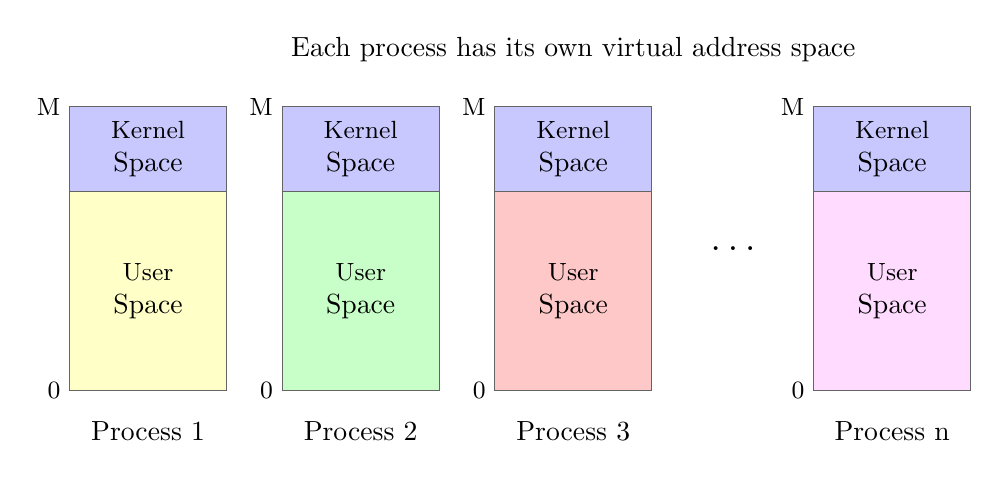
\begin{tikzpicture}[scale=0.9]
    % Define colors
    \definecolor{kernelcolor}{RGB}{200,200,255}
    \definecolor{usercolor1}{RGB}{255,255,200}
    \definecolor{usercolor2}{RGB}{200,255,200}
    \definecolor{usercolor3}{RGB}{255,200,200}
    \definecolor{usercolor4}{RGB}{255,220,255}
    \definecolor{bordercolor}{RGB}{100,100,100}
    
    % Define dimensions
    \def\procwidth{2.2}
    \def\procheight{4}
    \def\kernelheight{1.2}
    \def\spacing{0.8}
    \pgfmathsetmacro{\kernelcenter}{\procheight-\kernelheight/2}
    \pgfmathsetmacro{\usercenter}{(\procheight-\kernelheight)/2}
    
    % Draw processes using foreach loop
    \foreach \i in {0, 1, 2} {
        \begin{scope}[shift={({\i*(\procwidth+\spacing)},0)}]
            \draw[thick, bordercolor] (0,0) rectangle (\procwidth,\procheight);
            
            % Kernel space (top)
            \fill[kernelcolor] (0,\procheight-\kernelheight) rectangle (\procwidth,\procheight);
            \draw[thick, bordercolor] (0,\procheight-\kernelheight) -- (\procwidth,\procheight-\kernelheight);
            
            % User space (bottom) - different color for each process
            \pgfmathtruncatemacro{\colornum}{\i+1}
            \fill[usercolor\colornum] (0,0) rectangle (\procwidth,\procheight-\kernelheight);
            
            % Labels with two lines
            \node[align=center] at (\procwidth/2, \kernelcenter) {\small Kernel\\Space};
            \node[align=center] at (\procwidth/2, \usercenter) {\small User\\Space};
            
            % Address labels
            \node[left] at (0, \procheight) {\small M};
            \node[left] at (0, 0) {\small 0};
            
            % Process label
            \pgfmathtruncatemacro{\procnum}{\i+1}
            \node[below] at (\procwidth/2, -0.3) {Process \procnum};
        \end{scope}
    }
    
    % Dots indicating more processes
    \node at ({{3*(\procwidth+\spacing) + \spacing/2}}, \procheight/2) {\Large \ldots};
    
    % Process n
    \begin{scope}[shift={({3.5*(\procwidth+\spacing)},0)}]
        \draw[thick, bordercolor] (0,0) rectangle (\procwidth,\procheight);
        
        % Kernel space (top)
        \fill[kernelcolor] (0,\procheight-\kernelheight) rectangle (\procwidth,\procheight);
        \draw[thick, bordercolor] (0,\procheight-\kernelheight) -- (\procwidth,\procheight-\kernelheight);
        
        % User space (bottom) - use color 4 for process n
        \fill[usercolor4] (0,0) rectangle (\procwidth,\procheight-\kernelheight);
        
        % Labels with two lines
        \node[align=center] at (\procwidth/2, \kernelcenter) {\small Kernel\\Space};
        \node[align=center] at (\procwidth/2, \usercenter) {\small User\\Space};
        
        % Address labels
        \node[left] at (0, \procheight) {\small M};
        \node[left] at (0, 0) {\small 0};
        
        % Process label
        \node[below] at (\procwidth/2, -0.3) {Process n};
    \end{scope}
    
    % Title/description
    \node[above, font=\normalsize] at ({2.5*\procwidth + 2*\spacing}, \procheight + 0.5) {Each process has its own virtual address space};
    
\end{tikzpicture}
\end{center}
\end{frame}

\begin{frame}{Virtual Memory: Basic Idea}
\begin{itemize}
\item \textbf{Basic terminology}
    \begin{itemize}
    \item Virtual Address Space (per process): address space used by the process
    \item Physical Address: actual physical memory address space
    \end{itemize}
\item \textbf{Divide each space (virtual and physical) into fixed size blocks}
    \begin{itemize}
    \item Pages in Virtual space, Frames in Physical space
    \item Page size = Frame size = some power of 2
    \end{itemize}
\item \textbf{Virtual pages are mapped either to}
    \begin{itemize}
    \item A physical frame in memory
    \item Or a sector in the disk
    \end{itemize}
\item \textbf{All addresses in programs use Virtual Memory Address Space}
    \begin{itemize}
    \item Hardware translates virtual to physical addresses on-the-fly
    \item Uses a Page Table for the translation
    \end{itemize}
\end{itemize}
\end{frame}

\begin{frame}{Page Tables}
\begin{itemize}
\item The OS manages a page table for each process
    \begin{itemize}
    \item The OS maps the process virtual pages to physical pages or to disk
    \item Only the OS writes into the page tables
    \item The page tables reside in the physical memory (DRAM)
    \end{itemize}
\end{itemize}
\begin{center}
[Diagram: Page Table mapping Virtual Pages to Physical Pages and Disk with Present bits]
\end{center}
\end{frame}

\begin{frame}{Virtual to Physical Address Translation}
\begin{itemize}
\item PTE – Page Table Entry
\item Page size: $2^{12}$ byte = 4K byte
\end{itemize}
\begin{center}
[Diagram showing virtual address (47-12 bits VPN, 11-0 bits offset) mapping to physical address]
\end{center}
Components:
\begin{itemize}
\item Page table base reg
\item Present bit, Dirty bit
\item Access Control (Memory type, User/Supervisor)
\item Physical page number
\end{itemize}
\end{frame}

\begin{frame}{Page Table Location}
\begin{itemize}
\item The page table of each process resides in main memory
    \begin{itemize}
    \item When a process is running, the start address of its page table is pointed by a special register in the CPU: the page table base register
    \item The page table base register holds the physical address of entry 0
    \end{itemize}
\item The physical address of the PTE of virtual page \#VPN
    \begin{itemize}
    \item PTE address = Page table base reg + VPN $\times$ PTE\_size
    \end{itemize}
\end{itemize}
\end{frame}

\begin{frame}{Mapping Virtual Address Spaces to Physical Memory}
\begin{itemize}
\item Each process has its own address space $\rightarrow$ each process has its own page table
    \begin{itemize}
    \item A process cannot access physical memory allocated to another process (unless OS intentionally shares some of it)
    \end{itemize}
\item On a context switch, the Page Table Base Register is loaded with the page table base address of the process that moves in
\end{itemize}
\begin{center}
[Diagram: Multiple process virtual address spaces mapping to physical memory]
\end{center}
\end{frame}

\begin{frame}{Page Fault and Protection Violation Fault}
\textbf{If present bit in the page table entry == 0 then // page fault}
\begin{itemize}
\item Page is not mapped to main memory $\rightarrow$ need to retrieve it from disk
\item The CPU detects the situation, but cannot remedy it $\rightarrow$ traps to the OS
\item The OS takes care of the page fault:
    \begin{itemize}
    \item If there is no free space in physical memory:
        \begin{itemize}
        \item Picks a physical page to discard (based on some replacement policy)
        \item Marks the page as not present in the page table
        \item Copies the page to the disk swap area
        \end{itemize}
    \item Loads the new page from disk into the selected physical page
    \item Updates the page table entry of the new page
    \item Resumes to the program so HW retries and succeeds
    \end{itemize}
\end{itemize}
\textbf{When a page is present the CPU checks the page access control bits}
\begin{itemize}
\item R = Read-only, R/W = read/write, X = execute only
\item If access type is not compatible with the specified access rights $\rightarrow$ protection violation fault
\end{itemize}
\end{frame}

\begin{frame}{Optimal Page Size}
\begin{itemize}
\item \textbf{Minimize wasted storage}
    \begin{itemize}
    \item Small pages minimize internal fragmentation
    \item Small pages increase the size of the page tables
    \end{itemize}
\item \textbf{Minimize transfer time – use large pages (multiple disk sectors)}
    \begin{itemize}
    \item Amortize access cost and prefetch useful data
    \item But, might transfer unnecessary data and discard (victimize) useful data
    \end{itemize}
\item \textbf{General trend toward larger pages because}
    \begin{itemize}
    \item Big cheap RAM
    \item Increasing memory / disk performance gap
    \item Larger address spaces
    \item Programs with larger code and data
    \end{itemize}
\end{itemize}
\end{frame}

\begin{frame}{Translation Look aside Buffer (TLB)}
\begin{itemize}
\item With virtual memory, before each cache access, need to first get the physical address
    \begin{itemize}
    \item The page table resides in memory $\rightarrow$ each translation requires an extra memory access
    \end{itemize}
\item The TLB is a cache for recent address translations
\end{itemize}
\begin{center}
[Diagram: TLB caching page table entries]
\end{center}
\end{frame}


\begin{frame}{Translation Look aside Buffer (TLB)}
\begin{columns}[T]
\begin{column}{0.55\textwidth}
\begin{itemize}
\item \textbf{The TLB caches recently used PTEs}
    \begin{itemize}
    \item Typically, 128 to 256 entries, 4 to 8 way associative
    \end{itemize}
    
\item \textbf{TLB Indexing}
\end{itemize}

\vspace{0.2cm}
\begin{center}
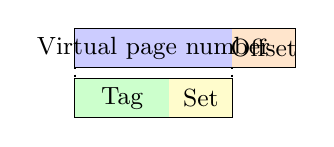
\begin{tikzpicture}[scale=0.8]
    % Virtual address breakdown
    \draw[thick] (0,0) rectangle (3.5,0.6);
    \draw[thick] (2.5,0) -- (2.5,0.6);
    
    % Fill colors
    \fill[blue!20] (0,0) rectangle (2.5,0.6);
    \fill[orange!20] (2.5,0) rectangle (3.5,0.6);
    
    % Labels
    \node at (1.25,0.3) {\small Virtual page number};
    \node at (3,0.3) {\small Offset};
    
    % Tag and Set subdivision
    \draw[thick] (0,-0.8) rectangle (2.5,-0.2);
    \draw[thick] (1.5,-0.8) -- (1.5,-0.2);
    
    \fill[green!20] (0,-0.8) rectangle (1.5,-0.2);
    \fill[yellow!20] (1.5,-0.8) rectangle (2.5,-0.2);
    
    \node at (0.75,-0.5) {\small Tag};
    \node at (2,-0.5) {\small Set};
    
    % Dotted lines connecting
    \draw[dotted, thick] (0,0) -- (0,-0.2);
    \draw[dotted, thick] (2.5,0) -- (2.5,-0.2);
\end{tikzpicture}
\end{center}

\vspace{0.3cm}
\begin{itemize}
\item \textbf{On A TLB miss}
    \begin{itemize}
    \item Page Miss Handler (HW PMH) injects a load to address PTBR+VPN$\times$PTE\_size to get the PTE from memory
    \item PMH may contain a 2\textsuperscript{nd} level TLB
    \end{itemize}
    
\item \textbf{OS is responsible to maintain coherency between page table and TLB}
    \begin{itemize}
    \item Each time OS writes to a PTE it must invalidate the PTE from the TLB (if exists)
    \end{itemize}
\end{itemize}
\end{column}

\begin{column}{0.45\textwidth}
\begin{center}
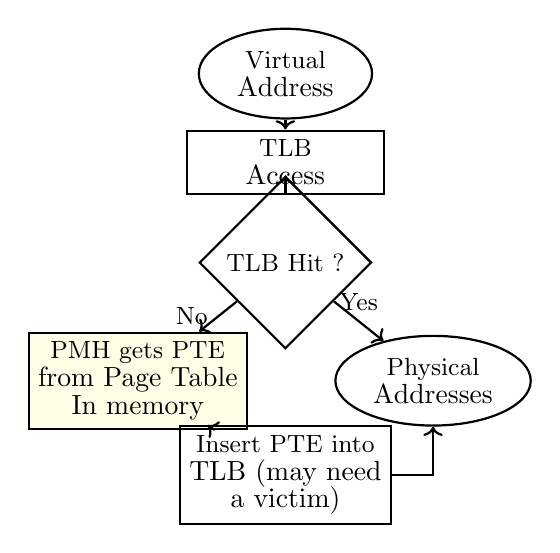
\begin{tikzpicture}[scale=0.75,
    box/.style={rectangle, draw, thick, minimum width=2.5cm, minimum height=0.7cm, text centered},
    decision/.style={diamond, draw, thick, minimum width=1.8cm, minimum height=1.2cm, text centered},
    oval/.style={ellipse, draw, thick, minimum width=2.2cm, minimum height=0.8cm, text centered},
    arrow/.style={->, thick}]
    
    % Nodes
    \node[oval, align=center] (va) at (0,6) {\small Virtual\\[-2pt] Address};
    \node[box, align=center] (tlb) at (0,4.5) {\small TLB\\[-2pt] Access};
    \node[decision] (hit) at (0,2.8) {\small TLB Hit ?};
    \node[box, fill=yellow!10, align=center] (pmh) at (-2.5,0.8) {\small PMH gets PTE\\[-2pt] from Page Table\\[-2pt] In memory};
    \node[box, align=center] (insert) at (0,-0.8) {\small Insert PTE into\\[-2pt] TLB (may need\\[-2pt] a victim)};
    \node[oval, align=center] (pa) at (2.5,0.8) {\small Physical\\[-2pt] Addresses};
    
    % Arrows
    \draw[arrow] (va) -- (tlb);
    \draw[arrow] (tlb) -- (hit);
    \draw[arrow] (hit) -- node[left] {\small No} (pmh);
    \draw[arrow] (hit) -- node[above] {\small Yes} (pa);
    \draw[arrow] (pmh) -- (insert);
    \draw[arrow] (insert) -| (pa);
    
\end{tikzpicture}
\end{center}
\end{column}
\end{columns}
\end{frame}

\begin{frame}{Translation Look aside Buffer (TLB) - Details}
\begin{itemize}
\item The TLB caches recently used PTEs
    \begin{itemize}
    \item Typically, 128 to 256 entries, 4 to 8 way associative
    \end{itemize}
\item \textbf{TLB Indexing}
\item \textbf{On A TLB miss}
    \begin{itemize}
    \item Page Miss Handler (HW PMH) injects a load to address PTBR+VPN$\times$PTE\_size to get the PTE from memory
    \item PMH may contain a 2nd level TLB
    \end{itemize}
\item OS is responsible to maintain coherency between page table and TLB
    \begin{itemize}
    \item Each time OS writes to a PTE it must invalidate the PTE from the TLB (if exists)
    \end{itemize}
\end{itemize}
\end{frame}

\begin{frame}{Processor Caches and TLBs}
\begin{itemize}
\item Each of L1 I\$ and L1 D\$ has its own TLB – ITLB and DTLB
    \begin{itemize}
    \item Similar to the I\$ and the D\$, the ITLB and DTLB are accessed in different pipe-stages
    \end{itemize}
\item In case of either ITLB or DTLB miss: access the STLB (second level TLB)
\item In case of STLB miss
    \begin{itemize}
    \item PMH (page miss handler) injects a load to get the PTE from the page table (page walk)
    \item This load, like any other load, starts by a lookup in the L1 D\$
    \end{itemize}
\end{itemize}
\begin{center}
[Diagram: Core with L1 I\$, L1 D\$, ITLB, DTLB, STLB, L2, L3, and Memory hierarchy]
\end{center}
\end{frame}

\begin{frame}{Virtual Memory And Cache}
\begin{itemize}
\item Page table entries are cached in L1 D\$, L2\$ and L3\$ as data
\item If the injected load misses in a cache $\rightarrow$ perform a cache line fill
    \begin{itemize}
    \item all PTEs in the missed cached line are brought into the cache
    \end{itemize}
\item Only the specific missed PTE is filled into the STLB and TLB
\end{itemize}
\textbf{Get the Translation:}
Virtual Page Number $\rightarrow$ TLB hit? $\rightarrow$ STLB hit? $\rightarrow$ PMH $\rightarrow$ L1\$/L2\$/L3\$/Mem

\textbf{Get the Data:}
PFN + offset $\rightarrow$ L1\$ hit? $\rightarrow$ L2\$ hit? $\rightarrow$ L3\$ hit? $\rightarrow$ Access Mem
\end{frame}

\begin{frame}{Overlapping TLB \& Cache Access}
\textbf{Goal:} start cache access in parallel to TLB access
\begin{itemize}
\item Save a cycle on getting the data in case of TLB hit and cache hit
\end{itemize}

\textbf{Cache \#set contained in page offset}
\begin{itemize}
\item Cache set available before translation
\item Access cache set in parallel with TLB
\item Once translation is done, match physical page number with tag of each way
\end{itemize}

\textbf{Restriction on cache}
\begin{itemize}
\item \#sets $\times$ line size = way size $\leq$ page size
\item Cache size $\leq$ page size $\times$ associativity
\end{itemize}
\end{frame}

\begin{frame}{Evicting a Page to Disk}
\textbf{OS updates the Page Table}
\begin{itemize}
\item OS invalidate the page from the TLBs (using a special instruction)
    \begin{itemize}
    \item It is the OS responsibility to maintain coherency between page table and TLBs for any change in the page table
    \end{itemize}
\item OS marks the swapped-out page as not present (present=0) in its PTE
    \begin{itemize}
    \item If the PTE is cached in any of the caches, MESI protocol maintains coherency
    \end{itemize}
\item OS writes the page disk location into the PTE
\end{itemize}

\textbf{OS copies the page to the disk}
\begin{itemize}
\item Read each block (=cache line) within the page
\item Snoop-invalidate each line in the CPUs caches
\item Write the block to the disk-controller Memory-Mapped I/O area
\end{itemize}
\end{frame}

\begin{frame}{Context Switch}
\textbf{On a context switch}
\begin{itemize}
\item Save the current architectural state to a dedicated memory location
    \begin{itemize}
    \item HW supports fast save command
    \item Architectural registers, including the page-table base-address register
    \end{itemize}
\item Flush the TLBs
\item Load the new architectural state from memory
    \begin{itemize}
    \item Architectural registers, including the page-table base-address register
    \end{itemize}
\end{itemize}
\end{frame}

\begin{frame}{Virtually-Addressed Cache}
\begin{itemize}
\item Cache uses virtual addresses (tags are virtual)
\item Address translation only done on a cache miss
    \begin{itemize}
    \item TLB is not in the path to cache hit
    \end{itemize}
\item Two virtual pages mapped to the same physical page
    \begin{itemize}
    \item Must not reside in the cache together
    \item On a cache miss, use a reverse TLB to verify that no other cache line already in the cache mapped to the missed physical address
    \end{itemize}
\item Flush cache on context switch
    \begin{itemize}
    \item Alternatively: add process ID as part of the tag
    \end{itemize}
\end{itemize}
\begin{center}
[Diagram: CPU $\rightarrow$ VA $\rightarrow$ Cache $\rightarrow$ TLB $\rightarrow$ PA $\rightarrow$ Main Memory]
\end{center}
\end{frame}

\begin{frame}{Paging in x86}
\begin{center}
\Huge Paging in x86
\end{center}
\end{frame}

\begin{frame}{Page Tables Size}
\textbf{Assume}
\begin{itemize}
\item A virtual address space of size $2^{48}$ bytes
\item A page size of 4KB = $2^{12}$B $\rightarrow$ $2^{48}$B / $2^{12}$B = $2^{36}$ entries in the page table
\item A PTE size of 8 bytes $\rightarrow$ page table size is $2^{36} \times 8$B = $2^{39}$B
\item 128 process running in the system, each with it own page table $\rightarrow$ $2^{39}$B $\times$ 128 = $2^{46}$B
\item Page tables alone requires a huge physical memory
\end{itemize}

\textbf{Solution}
\begin{itemize}
\item Most processes use a small portion of the virtual address space
\item Use hierarchical page tables – the page table of each process maps the pages that the process is actually using (allocated to), and not the entire virtual address space
\item The hierarchical page table is split into pages
\item Some of the pages in the page table hierarchy may be not in physical memory
    \begin{itemize}
    \item In case getting to such a page, the CPU traps to the OS to get the page
    \end{itemize}
\end{itemize}
\end{frame}

\begin{frame}{4KB Page Mapping in 64-bit Mode}
\textbf{Hierarchical mapping}
\begin{itemize}
\item The size of each page table is 4KB (in each hierarchy)
\item Each page table entry has 8 bytes
\item Each page table has 4KB/8B = 512 entries
\item The page table entry of level N provides the base of the page table in level N-1
    \begin{itemize}
    \item Provides M-12 bits, bit[11:0] are zeros (aligned to the 4KB table size)
    \item M is log2 of physical memory size
    \item CR3 points to PML4 table base
    \end{itemize}
\item 9 bits from the VA provide the index for the specific entry in the page table
\end{itemize}
\textbf{Lowest 12 Linear Addr. bits provide offset within the selected 4KB page}
\begin{itemize}
\item Point to the data bytes
\end{itemize}
\end{frame}

\begin{frame}{Example: Page Table Hierarchy}
\begin{center}
[Complex diagram showing page table hierarchy with PML4, PDP, DIR, TABLE levels and address mappings]
\end{center}
This example shows how the OS dynamically allocates page tables in the page table hierarchy, as more addresses are requested by a process
\end{frame}

\begin{frame}{2MB Page Mapping in 64-bit Mode}
\textbf{A page directory entry (an entry for the 2nd level tables) has a "page size" bit}
\begin{itemize}
\item \textbf{If page size = 1}
    \begin{itemize}
    \item The entry points to a 2M page
    \item Address bits[20:0] are used as an offset within the 2MB page
    \end{itemize}
\item \textbf{If page size = 0}
    \begin{itemize}
    \item The entry points to the base of a page table (1st level table)
    \item That page table maps 512 pages of size 4KB, for a total size of 512$\times$4KB = 2MB
    \item Address bits[20:12] select an entry within 1st level table
    \item Address bits[11:0] are used as an offset within the selected 4KB page
    \end{itemize}
\end{itemize}
\end{frame}

\begin{frame}{1GB Page Mapping in 64-bit Mode}
\textbf{A PDP entry (an entry for the 3rd-level tables) has a "page size" bit}
\begin{itemize}
\item \textbf{If page size = 1}
    \begin{itemize}
    \item The entry points to a 1GB page
    \item Address bits[29:0] are used as an offset within the 1GB page
    \end{itemize}
\item \textbf{If page size = 0}
    \begin{itemize}
    \item The entry points to the base of a page directory table (2nd-level table)
    \item That page directory table maps a total of 1GB
    \end{itemize}
\end{itemize}
\end{frame}

\begin{frame}{PTE/PDE/PDP/PML4 Entry Format}
\begin{itemize}
\item \textbf{Physical frame address}
\item \textbf{Virtual memory}
    \begin{itemize}
    \item Present – page is mapped to phys. mem
    \item Accessed – page data was accessed
    \item Dirty – data in page was modified
    \item Global – remains in TLB on context sw.
    \item Page size – in hierarchies 2 and up
    \end{itemize}
\item \textbf{Protection}
    \begin{itemize}
    \item R\#/W – page is read only / writable
    \item User / Supervisor\# – page can be accessed by user+OS or by OS only
    \item eXecute Disable – page can be used only as data (fault if trying to execute)
    \end{itemize}
\item \textbf{Caching}
    \begin{itemize}
    \item PWT – Page Write Through
    \item PCD – Page Cache Disabled
    \item PAT – PT Attribute Index
    \end{itemize}
\item \textbf{Ignored} – bits available for OS usage
\end{itemize}
\end{frame}

\begin{frame}{TLBs}
\textbf{The most recently used PDEs and PTEs are cached in TLBs}
\begin{itemize}
\item Separate TLB for data and instruction caches
\item Separate TLBs for 4KB, 2/4MB and 1GB page sizes
\item 2nd level TLB serves both instruction TLB and data TLB
\item TLB sizes in 6th Generation Intel® Core™ Processors:
\end{itemize}

\begin{center}
\footnotesize
\begin{tabular}{|l|c|c|c|}
\hline
 & \textbf{4KB pages} & \textbf{2MB/4MB Pages} & \textbf{1GB Pages} \\
\hline
Instruction TLBs & 128 entries, 8 ways & 8 entries / thread & none \\
\hline
Data TLBs & 64 entries, 4 ways & 32 entries, 4 ways & 4 entries, 4 ways \\
\hline
2nd level TLB & \multicolumn{2}{c|}{1536 entries, 12 ways (Shared by 4KB and 2/4MB pages)} & 16 entries, 4 ways \\
\hline
\end{tabular}
\end{center}

\textbf{In case of a hit in multiple TLBs}
\begin{itemize}
\item The largest page that hits is used
\end{itemize}
\end{frame}

\begin{frame}{PMH – Page Miss Handler}
\textbf{In case of an iTLB or a dTLB miss $\rightarrow$ Request PTE from PMH}
\begin{itemize}
\item PMH first tries the STLB (2nd level TLB) – save walk in case of an STLB hit
\item If STLB miss, PMH performs a page-walk: traverses the page table tree, starting at the root
\end{itemize}

\textbf{The PMH includes caches to shorten the page walk time}
\begin{itemize}
\item All 3 caches are accessed in parallel – use hit from the lowest table that hits
\item For each table that needs memory access PMH injects a "load"
\end{itemize}

\begin{center}
\footnotesize
\begin{tabular}{|l|l|l|l|}
\hline
\textbf{cache} & \textbf{Accessed with VA bits} & \textbf{If hits, returns} & \textbf{saves accesses to tables} \\
\hline
PDE cache & [47:21] & PDE & PTE \\
PDP cache & [47:30] & PDP entry & PDE and PTE \\
PML4 cache & [47:39] & PML4 entry & PDP, PDE, and PTE \\
\hline
\end{tabular}
\end{center}

\textbf{Page attributes}
\begin{itemize}
\item R/W flag: logical AND of R/W flag in all levels
\item U/S flag: logical OR of U/S flag in all levels
\item XD flag: logical OR of XD flag in all levels
\end{itemize}
\end{frame}

\begin{frame}{PMH: Page Walk Flowchart}
\begin{center}
[Complex flowchart showing page walk process with TLB hit, STLB hit, and various cache lookups]
\end{center}
\end{frame}

\begin{frame}{Translation Page Not Present}
\textbf{During a page walk, a translation hierarchy may return an entry with Present = 0}
\begin{itemize}
\item The page of translations pointed by this entry is not present in memory
\item PMH gets a page fault $\rightarrow$ the original load (not the PMH-injected load) faults to the OS
\item OS gets the missing translation page into memory
\item The load is re-fetched (and the PMH performs the walk again)
    \begin{itemize}
    \item The OS uses unused bits in the entry to encode the page location in the disk
    \item Most likely the lower pages in the hierarchy are also not be present
    \item OS brings all missing pages as part handling the same page fault
    \end{itemize}
\end{itemize}

\textbf{CR3 does not have a "present" bit}
\begin{itemize}
\item The PML4 table, which uses a single 4K page, is always present
\end{itemize}
\end{frame}

\begin{frame}{Cache and Translation Structures}
\begin{center}
[Diagram showing Core with PMH, L1 I\$ 32KB 8 ways, L1 D\$ 32KB 8 ways, MLC 256KB 4 ways, LLC 2MB per core, DRAM 8GB, and various TLB structures]
\end{center}
\end{frame}

% Backup slides section
\section{Backup}

\begin{frame}{Backup}
\begin{center}
\Huge Backup
\end{center}
\end{frame}

\begin{frame}{Why Virtual Memory?}
\begin{itemize}
\item \textbf{Generality} – ability to run programs larger than size of physical memory
\item \textbf{Storage management} – allocation/deallocation of variable sized blocks is costly and leads to (external) fragmentation
\item \textbf{Protection} – regions of the address space can be R/O, Ex, ...
\item \textbf{Flexibility} – portions of a program can be placed anywhere, without relocation
\item \textbf{Storage efficiency} – retain only most important portions of the program in memory
\item \textbf{Concurrent I/O} – execute other processes while loading/dumping page
\item \textbf{Expandability} – can leave room in virtual address space for objects to grow
\item \textbf{Performance}
\end{itemize}
\end{frame}

\begin{frame}{Page Aliasing}
\textbf{OS may map different virtual pages to the same physical page}

\textbf{DLLs in Linux/Windows}
\begin{itemize}
\item DLL pages are used by all processes, marked as read only
\item Same DLL may be loaded by a process more than once
\end{itemize}

\textbf{Large malloc – Copy-on-Write}
\begin{itemize}
\item OS maps all allocated virtual pages to the same all-zero physical page
\item The newly allocated virtual page is marked as read-only in its PTE
\item In case of a write to one of these virtual pages:
    \begin{itemize}
    \item Get access violation page-fault
    \item OS identifies that the page is mapped to the special physical page
    \item OS allocates a "real" physical page (copy-on-write)
    \end{itemize}
\end{itemize}

\textbf{Shared Memory}
\begin{itemize}
\item OS maps virtual pages of different processes to the same physical page
\end{itemize}
\end{frame}

\begin{frame}{32bit Mode: 4KB Page Mapping}
\textbf{2-level hierarchical mapping}
\begin{itemize}
\item Page directory and page tables
\item Pages / page tables are 4KB aligned
\end{itemize}

\begin{itemize}
\item CR3 points to the current Page Directory
\item Upper 10 Linear addr. bits point to a PDE
    \begin{itemize}
    \item PDE provides a 20 bit, 4KB aligned base physical address of a page table
    \end{itemize}
\item Next 10 Linear addr. bits point to a PTE within the given Page Table
    \begin{itemize}
    \item PTE provides a 20 bit, 4KB aligned, base physical address of a 4KB page
    \end{itemize}
\item Lowest 12 Linear Addr. bits provide offset within the selected 4KB page
\end{itemize}
\end{frame}

\begin{frame}{32bit Mode: 4MB Page Mapping}
\begin{itemize}
\item PDE directly maps up to 1024 4MB pages
\item Upper 10 Linear addr. bits point to a PDE
    \begin{itemize}
    \item PS in the PDE = 1
    \item PDE provides a 10 bit, 4MB aligned, base physical address of a 4MB page
    \end{itemize}
\item Lowest 22 Linear addr. bits provide offset within selected 4MB page
\end{itemize}

\textbf{Mixing 4KByte and 4MByte Pages}
\begin{itemize}
\item Separate TLBs for 4MB pages and 4KB pages
    \begin{itemize}
    \item Often-used code (e.g., kernels) is placed in a 4MB page $\rightarrow$ frees up 4KB TLB entries
    \item Reduces TLB misses and improve overall system performance
    \end{itemize}
\end{itemize}
\end{frame}

\begin{frame}{PAE – Physical Address Extension}
\textbf{When PAE (physical address extension) flag in CR4 is set}
\begin{itemize}
\item Physical addresses is extended to M bits
    \begin{itemize}
    \item Linear address remains 32 bit
    \end{itemize}
\item Each page table entry becomes 64 bits to hold the extra phy. address bits
    \begin{itemize}
    \item Page directory and page tables remain 4KB in size
    \item Number of entries in each table is halved to 512
    \item Indexed by 9 instead of 10 bits
    \end{itemize}
\end{itemize}

\textbf{A new 4 entry Page Directory Pointer Table is added}
\begin{itemize}
\item Indexed by bits [31:30] of the linear address
\item Each entry points to a page directory
\item CR3 contains the page-directory-pointer-table base address
    \begin{itemize}
    \item Provides the m.s.bits of the physical address
    \item Forcing the table to be located on a 32-byte boundary
    \end{itemize}
\end{itemize}
\end{frame}

\begin{frame}{Execute-Disable Bit}
\textbf{Supported only with PAE enabled / 64 bit mode}
\begin{itemize}
\item Bit[63] in PML4 entry, PDP entry, PDE, PTE
\end{itemize}

\textbf{If the execute disable bit of a memory page is set}
\begin{itemize}
\item The page can be used only as data
\item An attempt to execute code from a memory page with the execute-disable bit set causes a page-fault exception
\item Setting the execute-disable bit at any level of the paging structure, protects all pages pointed from this entry
\end{itemize}
\end{frame}

\begin{frame}{Page Table – Virtual Mem. Attributes}
\textbf{Present (P) flag}
\begin{itemize}
\item When set: page is in physical memory
\item When clear, page not in memory $\rightarrow$ processor generates a page-fault
\item The processor does not set/clear this flag – OS maintains its state
\item In case of a page-fault, the OS performs the following operations:
    \begin{enumerate}
    \item Copy the page from disk into physical memory
    \item Load page address into PTE/PDE; set present=1, dirty=0, accessed=0
    \item Invalidate victim page from TLB
    \item Return from page-fault handler and restart the program
    \end{enumerate}
\end{itemize}

\textbf{Page size (PS) flag, in PDEs only}
\begin{itemize}
\item 0: The PDE points to a page table of 4KBytes pages
\item 1: The PDE points to a 4MB page
\end{itemize}
\end{frame}

\begin{frame}{Page Table – Virtual Mem. Attributes (cont.)}
\textbf{Accessed (A) flag and Dirty (D) flag}
\begin{itemize}
\item Typically cleared by the OS when a page/PT initially loaded into physical mem
\item Processor sets the A-flag the first time a page/PT is accessed (read/write)
\item Processor sets the D-flag the first time a page is accessed for a write
    \begin{itemize}
    \item The D-flag is not used in PDEs which point to page tables
    \end{itemize}
\item Both A and D flag are sticky
    \begin{itemize}
    \item Once set, the processor does not implicitly clear it – only software can clear it
    \end{itemize}
\item Used by OS to manage transfer of pages/PTs tables into and out of physical memory
\end{itemize}

\textbf{Global (G) flag}
\begin{itemize}
\item Indicates a global page when set (+ page global enable is set: CR4.PGE =1)
\item PTE/PDE in TLB not invalidated when CR3 is loaded / task switch
\item Only software can set or clear this flag
\end{itemize}
\end{frame}

\begin{frame}{Page Table – Caching Attributes}
\textbf{Page-level write-through (PWT) flag}
\begin{itemize}
\item Controls the write-through or write-back caching policy of the page / PT
    \begin{itemize}
    \item 0 : write-back caching, 1: write-through caching
    \end{itemize}
\item Ignored if the CD (cache disable) flag in CR0 is set
\end{itemize}

\textbf{Page-level cache disable (PCD) flag}
\begin{itemize}
\item Controls the caching of individual pages/PT
\item 1: caching of the associated page/PT is prevented
\item 0: the page/PT can be cached
\item Ignored (assumes as set) if the CD (cache disable) flag in CR0 is set
\end{itemize}

\textbf{Page table attribute index (PAT) flag}
\begin{itemize}
\item Used along with the PCD and PWT flags to select an entry in the PAT
\item Which in turn selects the memory type for the page
\end{itemize}
\end{frame}

\begin{frame}{Page Table – Protection Attributes}
\textbf{Read/write (R/W) flag}
\begin{itemize}
\item Specifies the read-write privileges for a page or group of pages
\item 0: the page is read only
\item 1: the page can be read and written into
\end{itemize}

\textbf{User/supervisor (U/S) flag}
\begin{itemize}
\item Specifies the user-supervisor privileges for a page or group of pages
\item 0: supervisor privilege level
\item 1: user privilege level
\end{itemize}
\end{frame}

\begin{frame}{Page Directory Base Address}
\textbf{The physical address of the page directory is stored in CR3 register}
\begin{itemize}
\item Also called the page directory base register (PDBR)
\end{itemize}

\textbf{PDBR is typically loaded with a new as part of a task switch}

\textbf{OS must ensure that}
\begin{itemize}
\item The page directory indicated by the PDBR image in a task's TSS (task state segment) is present in physical memory before the task is dispatched
\item The page directory must also remain in memory as long as the task is active
\end{itemize}
\end{frame}

\begin{frame}{TLBs}
\textbf{OS running at privilege level 0 can invalidate TLB entries}
\begin{itemize}
\item INVLPG instruction invalidates a specific PTE in the TLB
    \begin{itemize}
    \item This instruction ignores the setting of the G flag
    \end{itemize}
\item Whenever a PDE/PTE is changed (also when present flag is set to 0)
    \begin{itemize}
    \item OS must invalidate the corresponding TLB entry
    \end{itemize}
\item All (non-global) TLBs are automatically invalidated when CR3 is loaded
\end{itemize}

\textbf{The global (G) flag prevents frequently used pages from being automatically invalidated in on a task switch}
\begin{itemize}
\item The entry remains in the TLB indefinitely
\item Only INVLPG can invalidate a global page entry
\end{itemize}
\end{frame}

\end{document}